\section{1174003 - Dwi Septiani Tsaniyah}

\subsection{Soal Teori}
Praktek teori penunjang yang dikerjakan total nilai 100 sebagai nilai terpisah dari praktek pada modul ini(nilai 5 per nomor kecuali nomor terakhir 30 sisanya merupakan penanganan error, untuk hari pertama) :
\begin{enumerate}
\item
Jelaskan kenapa file teks harus di lakukan tokenizer. dilengkapi dengan ilustrasi atau gambar. \hfill \break
Tokenizer diperlukan untuk perhitungan bobot pada setiap teks karena Tokenizer akan membagi kalimat menjadi beberapa teks sehingga nantinya kalimat yang dimasukkan otomatis langsung diubah menjadi kata - kata dan akan dinilai sehingga akan memunculkan nilai vektor untuk digunakan saat prediksi teks yang muncul pada satu kalimat tersebut. Biasanya untuk memisahkan sebuah kata, tokenizer akan menggunakan spasi sebagai pemisah antar kata.
\begin{figure}[H]
    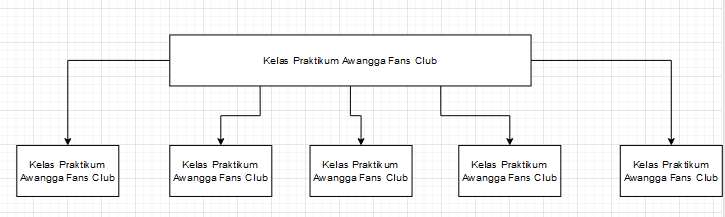
\includegraphics[width=4cm]{figures/1174003/7/teori_1.png}
    \centering
    \caption{Illustrasi Tokenizer}
\end{figure}
\item
Jelaskan konsep dasar K Fold Cross Validation pada dataset komentar Youtube pada kode listing \ref{lst:7.0}.dilengkapi dengan ilustrasi atau gambar.
\begin{lstlisting}[caption=K Fold Cross Validation,label={lst:7.0}]
kfold = StratifiedKFold(n_splits=5)
splits = kfold.split(d, d['CLASS'])
\end{lstlisting}
Pada koding diatas terdapat variabel kfold yang didalamnya berisi parameter split yang diisikan nilai 5. hal tersebut dimaksudkan untuk membuat pengolahan data akan diulang setiap datanya sebanyak lima kali dengan atribut class sebagai acuan pengolahan datanya. Lalu kemudian akan di hasilkan akurasi dari pengulangan data tersebut sebesar sekian persen tergantung datanya
\begin{figure}[H]
    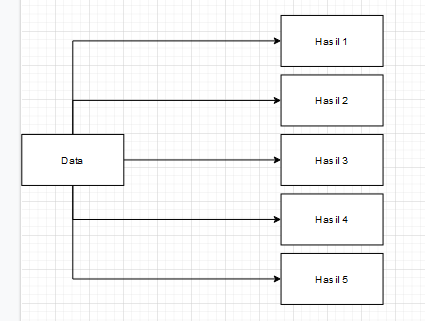
\includegraphics[width=4cm]{figures/1174003/7/teori_2.png}
    \centering
    \caption{Illustrasi K Fold Cross Validation}
\end{figure}
\item
Jelaskan apa maksudnya kode program \emph{for train, test in splits}.dilengkapi dengan ilustrasi atau gambar.
For train digunakan untuk melakukan training atau pelatihan pada data yang sudah dideklarasikan sebelumnya. Sedangkan test in split digunakan untuk membatasi jumlah data yang akan diinputkan atau data yang akan digunakan.
\item
Jelaskan apa maksudnya kode program \emph{train\_content = d['CONTENT'].iloc[train\_idx]} dan \emph{test\_content = d['CONTENT'].iloc[test\_idx]}. dilengkapi dengan ilustrasi atau gambar.
Maksud dari kode program tersebut adalah membaca isian kolom pada field yang bernama CONTENT sebagai data training dan data testing untuk program 
\begin{figure}[H]
    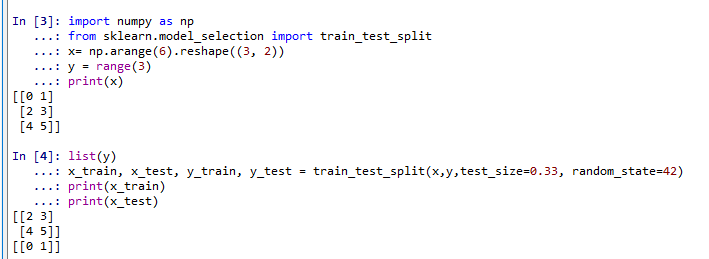
\includegraphics[width=4cm]{figures/1174003/7/teori_3.png}
    \centering
    \caption{Illustrasi For train dan test in split}
\end{figure}
\begin{figure}[H]
    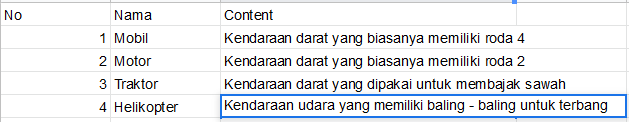
\includegraphics[width=4cm]{figures/1174003/7/teori_4.png}
    \centering
    \caption{Illustrasi penggunaan kolom Content}
\end{figure}
\item
Jelaskan apa maksud dari fungsi \emph{tokenizer = Tokenizer(num\_words=2000)} dan \emph{tokenizer.fit\_on\_texts(train\_content)}, dilengkapi dengan ilustrasi atau gambar.
\begin{itemize}
    \item tokenizer = Tokennizer(num\_words=2000) digunakan untuk membaca kalimat yang telah dibuat menjadi token sebanyak 2000 kata
    \item fit\_on\_texts digunakan untuk membuat membaca data token teks yang telah dimasukan kedalam fungsi yaitu fungsi train\_konten
\end{itemize}
\begin{figure}[H]
    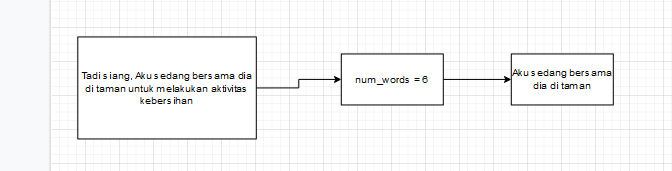
\includegraphics[width=4cm]{figures/1174003/7/teori_5.png}
    \centering
    \caption{Illustrasi fit tokenizer dan num\_word=2000}
\end{figure}
\item
Jelaskan apa maksud dari fungsi \emph{d\_train\_inputs = tokenizer.texts\_to\_matrix(train\_content, mode='tfidf')} dan \emph{d\_test\_inputs = tokenizer.texts\_to\_matrix(test\_content, mode='tfidf')}, dilengkapi dengan ilustrasi kode dan atau gambar.
Untuk digunakan sebagai pengubah urutan teks yang tadi telah dilakukan tkoenizer menjadi matriks yang berurutan seperti tf idf
\begin{figure}[H]
    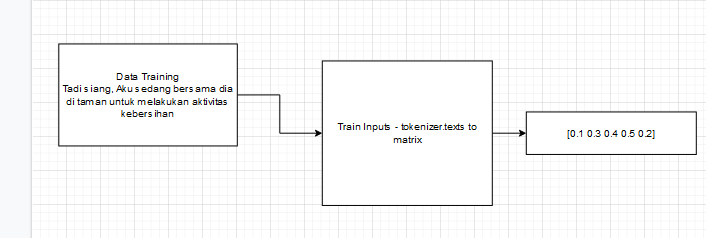
\includegraphics[width=4cm]{figures/1174003/7/teori_6.png}
    \centering
    \caption{Illustrasi d train inputs = tokenizer.texts to matrix}
\end{figure}
\item
Jelaskan apa maksud dari fungsi \emph{d\_train\_inputs = d\_train\_inputs/np.amax(np.absolute(d\_train\_inputs))} dan \emph{d\_test\_inputs = d\_test\_inputs/np.amax(np.absolute(d\_test\_inputs))}, dilengkapi dengan ilustrasi atau gambar.
Fungsi tersebut digunakan untuk membagi matriks tfidf dnegan penentuan maksimum array sepanjang sumbu sehingga akan menimbulkan garis ke bawah dan ke atas yang membentuk gambar v. Lalu hasil tersebut akan dimasukkan ke variabel d train input dan d test input dengan methode absolute. Yang berarti tanpa bilangan negatif.
\item
Jelaskan apa maksud fungsi dari \emph{d\_train\_outputs = np\_utils.to\_categorical(d['CLASS'].iloc[train\_idx])} dan \emph{d\_test\_outputs = np\_utils.to\_categorical(d['CLASS'].iloc[test\_idx])} dalam kode program, dilengkapi dengan ilustrasi atau gambar.
Maksud dari fungsi tersebut yaitu untuk merubah nilai vektor yang ada pada atribut class menjadi bentuk matrix dengan pengurutan berdasarkan data index training dan testing.
\item
Jelaskan apa maksud dari fungsi di listing \ref{lst:7.1}. Gambarkan ilustrasi Neural Network nya dari model kode tersebut.
\begin{lstlisting}[caption=Membuat model Neural Network,label={lst:7.1}]
       model = Sequential()
       model.add(Dense(512, input_shape=(2000,)))
       model.add(Activation('relu'))
       model.add(Dropout(0.5))
       model.add(Dense(2))
       model.add(Activation('softmax'))
\end{lstlisting}
model = sequential berarti variabel model berisi method sequential yang berguna untuk searching data dengan menerima parameter atau argumen kunci dengan langkah tertentu untuk mencari data yang telah diolah. Kemudian model akan ditambahkan method add dengan dense yang berarti data - data yang diinputkan akan terhubung, dengan data 612 dan 2000 data kata atau word kemudian model tersebut di masukan fungsi activation dengan rumus atau metode relu. setelah itu data akan di dropout 0.5atau dipangkas sebanyak 50 persen dikarenakan pada pohon bobot terlalu akurat terhadap data.
\begin{figure}[H]
    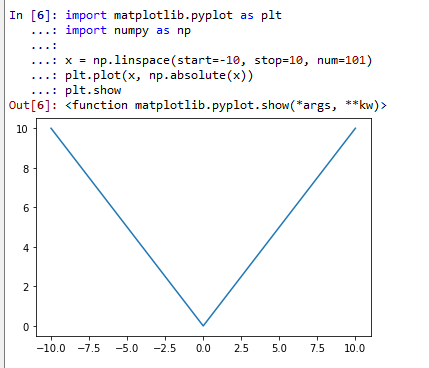
\includegraphics[width=4cm]{figures/1174003/7/teori_7.png}
    \centering
    \caption{Illustrasi d train inputs}
\end{figure}
\begin{figure}[H]
    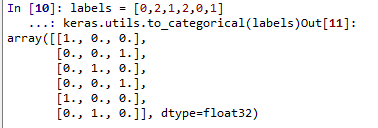
\includegraphics[width=4cm]{figures/1174003/7/teori_8.png}
    \centering
    \caption{Illustrasi train outputs = np utils.to categorical}
\end{figure}
\item
Jelaskan apa maksud dari fungsi di listing \ref{lst:7.2} dengan parameter tersebut.
\begin{lstlisting}[caption=Compile model,label={lst:7.2}]
	model.compile(loss='categorical_crossentropy', optimizer='adamax',
	                  metrics=['accuracy'])
\end{lstlisting}
model tersebut kemudian di compile atau di kembalikan kembali fungsi nilainya yangmana akan mengembalikan fungsi nilai loss nya berapa yang diambil dari fungsi adamax yang berberguna untuk mengetahui nilai lossnya kemudian metrics = acuracy merupakan akurasi dari nilai matrixnya. kemudian terdiri atas beberapa layer atau hiden layer. perbedaan antara deep learning dan DNN atau Deep Neural Network yaitu deep lerning merupakan pemakai algoritma dari DNN dan DNN merupakan algoritma yang ada pada deep learning.
\begin{figure}[H]
    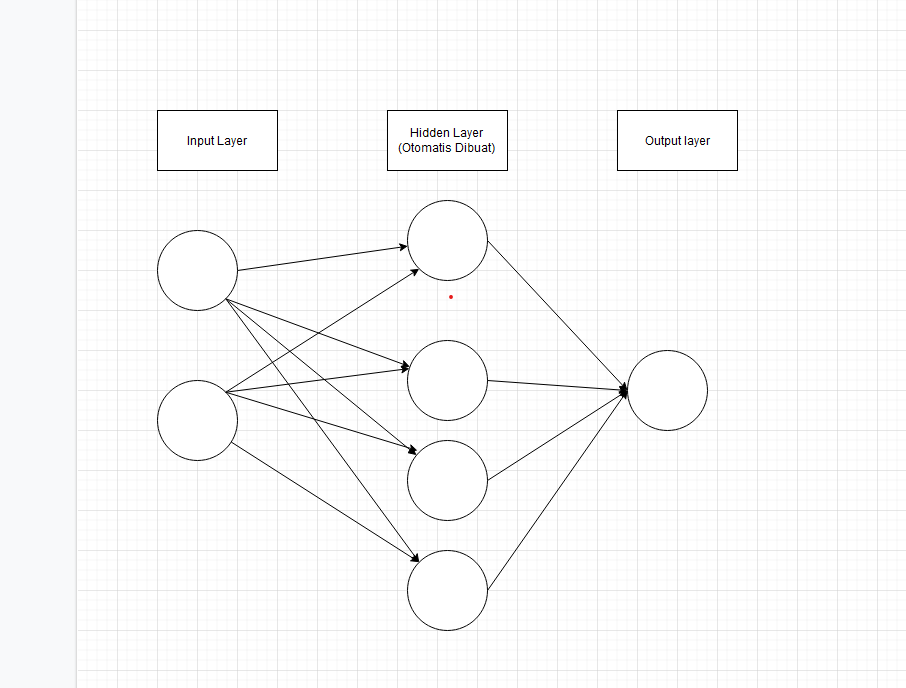
\includegraphics[width=4cm]{figures/1174003/7/teori_9.png}
    \centering
    \caption{Illustrasi Neural Network}
\end{figure}
\item
Jelaskan apa itu Deep Learning
Deep learning merupakan salah satu algoritma yang seperti Neural Network yang menggunakan meta data sebagai inputan dan mengolahnya menggunakan layer layer yang tersembunyi.
\item
Jelaskan apa itu Deep Neural Network, dan apa bedanya dengan Deep Learning
Deep Neural Network merupakan algoritma jaringan syaraf yang melakukan pembobotan terhadap data yang sudah ada sebagai acuan untuk data inputan selanjutnya. 
\item
Jelaskan dengan ilustrasi gambar buatan sendiri(langkah per langkah) bagaimana perhitungan algoritma konvolusi dengan ukuran stride (NPM mod3+1) x (NPM mod3+1) yang terdapat max pooling.(nilai 30)
sebelum membuat ilustrasi perlu di ketahui apa itu stride, stride adalah acuan atau parameter yang menentukan pergeseran pada filter fixcel. sebagai contoh nilai stride 1 yang berarti filter akan bergeser sebanyak satu fixcel secara vertikal dan horizontal. selanjutnya apa itu max pooling contoh pada suatu gambar di tentukan Max Pooling dari 3 x 3 dengan stride 1 yang berarti setiap pergeseran 1 pixcel akan diambil nilai terbesar dari pixcel 3 x 3 tersebut.
\begin{figure}[H]
    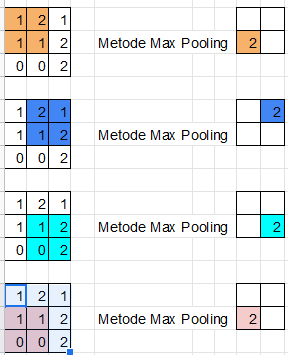
\includegraphics[width=4cm]{figures/1174003/7/teori_10.png}
    \centering
    \caption{Illustrasi perhitungan stride 1 max pooling}
\end{figure}
\end{enumerate}



\subsection{Praktek Program}
Tugas nilai terpisah dari teori maksimal 100. Praktekkan dan jelaskan dengan menggunakan bahasa yang mudah dimengerti dan bebas plagiat dan wajib skrinsut dari komputer sendiri masing masing nomor di bawah ini(nilai 5 masing masing pada hari kedua). Buka kode program pada repo Python-Artificial-Intelligence-Projects-for-Beginners pada github awangga. Buka folder Chapter04 file MathSymbols.py

\begin{enumerate}
\item Jelaskan kode program pada blok \# In[1]. Jelaskan arti dari setiap baris kode yang dibuat(harus beda dengan teman sekelas) dan hasil luarannya dari komputer sendiri.
\lstinputlisting[firstline=1, lastline=8]{src/1174003/7/chapter7.py}
\begin{figure}[H]
    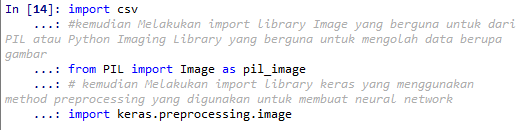
\includegraphics[width=4cm]{figures/1174003/7/praktek_1.png}
    \centering
    \caption{Illustrasi perhitungan stride 1 max pooling}
\end{figure}
\item Jelaskan kode program pada blok \# In[2]. Jelaskan arti dari setiap baris kode yang dibuat(harus beda dengan teman sekelas) dan hasil luarannya dari komputer sendiri.
\lstinputlisting[firstline=9, lastline=36]{src/1174003/7/chapter7.py}
\begin{figure}[H]
    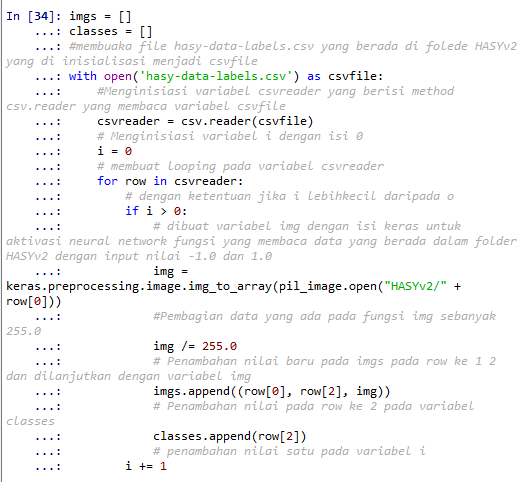
\includegraphics[width=4cm]{figures/1174003/7/praktek_2.png}
    \centering
    \caption{Illustrasi perhitungan stride 1 max pooling}
\end{figure}
\item Jelaskan kode program pada blok \# In[3]. Jelaskan arti dari setiap baris kode yang dibuat(harus beda dengan teman sekelas) dan hasil luarannya dari komputer sendiri.
\lstinputlisting[firstline=37, lastline=48]{src/1174003/7/chapter7.py}
\begin{figure}[H]
    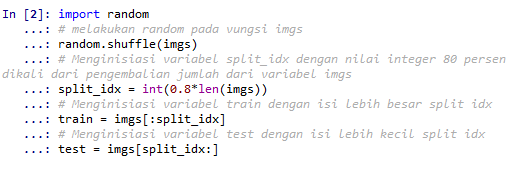
\includegraphics[width=4cm]{figures/1174003/7/praktek_3.png}
    \centering
    \caption{Illustrasi perhitungan stride 1 max pooling}
\end{figure}
\item Jelaskan kode program pada blok \# In[4]. Jelaskan arti dari setiap baris kode yang dibuat(harus beda dengan teman sekelas) dan hasil luarannya dari komputer sendiri.
\lstinputlisting[firstline=49, lastline=60]{src/1174003/7/chapter7.py}
\begin{figure}[H]
    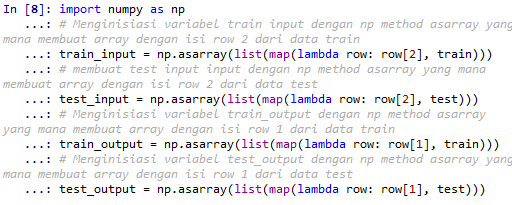
\includegraphics[width=4cm]{figures/1174003/7/praktek_4.png}
    \centering
    \caption{Illustrasi perhitungan stride 1 max pooling}
\end{figure}
\item Jelaskan kode program pada blok \# In[5]. Jelaskan arti dari setiap baris kode yang dibuat(harus beda dengan teman sekelas) dan hasil luarannya dari komputer sendiri.
\lstinputlisting[firstline=61, lastline=66]{src/1174003/7/chapter7.py}
\begin{figure}[H]
    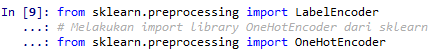
\includegraphics[width=4cm]{figures/1174003/7/praktek_5.png}
    \centering
    \caption{Illustrasi perhitungan stride 1 max pooling}
\end{figure}
\item Jelaskan kode program pada blok \# In[6]. Jelaskan arti dari setiap baris kode yang dibuat(harus beda dengan teman sekelas) dan hasil luarannya dari komputer sendiri.
\lstinputlisting[firstline=67, lastline=73]{src/1174003/7/chapter7.py}
\begin{figure}[H]
    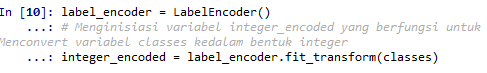
\includegraphics[width=4cm]{figures/1174003/7/praktek_6.png}
    \centering
    \caption{Illustrasi perhitungan stride 1 max pooling}
\end{figure}
\item Jelaskan kode program pada blok \# In[7]. Jelaskan arti dari setiap baris kode yang dibuat(harus beda dengan teman sekelas) dan hasil luarannya dari komputer sendiri.
\lstinputlisting[firstline=74, lastline=81]{src/1174003/7/chapter7.py}
\begin{figure}[H]
    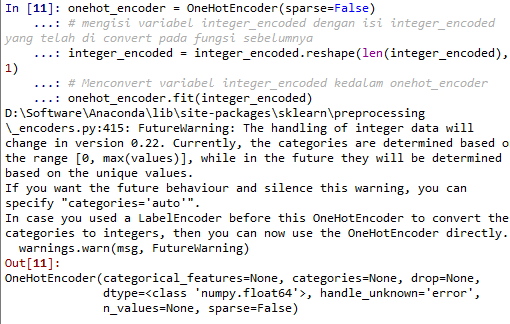
\includegraphics[width=4cm]{figures/1174003/7/praktek_7.png}
    \centering
    \caption{Illustrasi perhitungan stride 1 max pooling}
\end{figure}
\item Jelaskan kode program pada blok \# In[8]. Jelaskan arti dari setiap baris kode yang dibuat(harus beda dengan teman sekelas) dan hasil luarannya dari komputer sendiri.
\lstinputlisting[firstline=82, lastline=95]{src/1174003/7/chapter7.py}
\begin{figure}[H]
    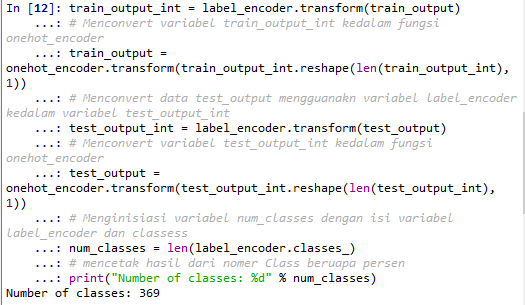
\includegraphics[width=4cm]{figures/1174003/7/praktek_8.png}
    \centering
    \caption{Illustrasi perhitungan stride 1 max pooling}
\end{figure}
\item Jelaskan kode program pada blok \# In[9]. Jelaskan arti dari setiap baris kode yang dibuat(harus beda dengan teman sekelas) dan hasil luarannya dari komputer sendiri.
\lstinputlisting[firstline=96, lastline=103]{src/1174003/7/chapter7.py}
\begin{figure}[H]
    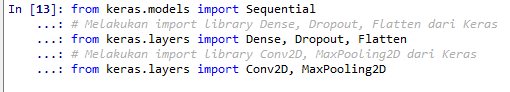
\includegraphics[width=4cm]{figures/1174003/7/praktek_9.png}
    \centering
    \caption{Illustrasi perhitungan stride 1 max pooling}
\end{figure}
\item Jelaskan kode program pada blok \# In[10]. Jelaskan arti dari setiap baris kode yang dibuat(harus beda dengan teman sekelas) dan hasil luarannya dari komputer sendiri.
\lstinputlisting[firstline=104, lastline=129]{src/1174003/7/chapter7.py}
\begin{figure}[H]
    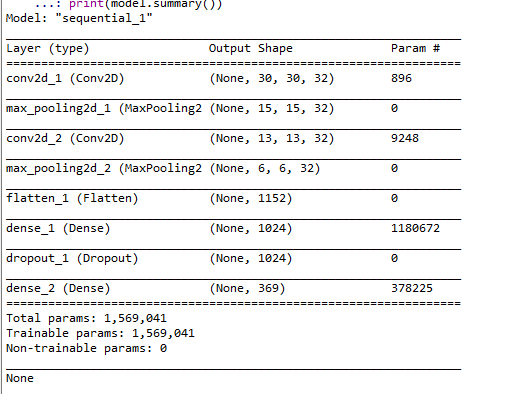
\includegraphics[width=4cm]{figures/1174003/7/praktek_10.png}
    \centering
    \caption{Illustrasi perhitungan stride 1 max pooling}
\end{figure}
\item Jelaskan kode program pada blok \# In[11]. Jelaskan arti dari setiap baris kode yang dibuat(harus beda dengan teman sekelas) dan hasil luarannya dari komputer sendiri.
\lstinputlisting[firstline=130, lastline=135]{src/1174003/7/chapter7.py}
\begin{figure}[H]
    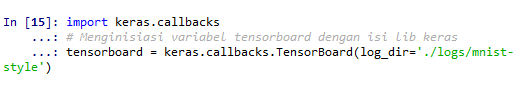
\includegraphics[width=4cm]{figures/1174003/7/praktek_11.png}
    \centering
    \caption{Illustrasi perhitungan stride 1 max pooling}
\end{figure}
\item Jelaskan kode program pada blok \# In[12]. Jelaskan arti dari setiap baris kode yang dibuat(harus beda dengan teman sekelas) dan hasil luarannya dari komputer sendiri.
\lstinputlisting[firstline=136, lastline=149]{src/1174003/7/chapter7.py}
\begin{figure}[H]
    \includegraphics[width=4cm]{figures/1174003/7/Praktek_12.png}
    \centering
    \caption{Illustrasi perhitungan stride 1 max pooling}
\end{figure}
\item Jelaskan kode program pada blok \# In[13]. Jelaskan arti dari setiap baris kode yang dibuat(harus beda dengan teman sekelas) dan hasil luarannya dari komputer sendiri.
\lstinputlisting[firstline=156, lastline=213]{src/1174003/7/chapter7.py}
\begin{figure}[H]
    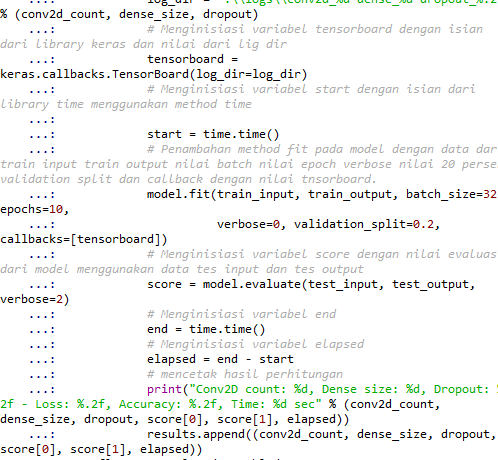
\includegraphics[width=4cm]{figures/1174003/7/praktek_13.png}
    \centering
    \caption{Illustrasi perhitungan stride 1 max pooling}
\end{figure}
\item Jelaskan kode program pada blok \# In[14]. Jelaskan arti dari setiap baris kode yang dibuat(harus beda dengan teman sekelas) dan hasil luarannya dari komputer sendiri.
\lstinputlisting[firstline=214, lastline=236]{src/1174003/7/chapter7.py}
\begin{figure}[H]
    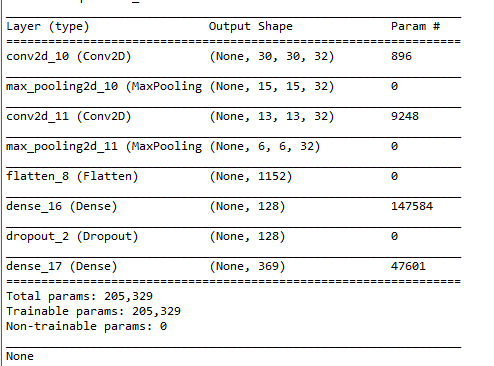
\includegraphics[width=4cm]{figures/1174003/7/praktek_14.png}
    \centering
    \caption{Illustrasi perhitungan stride 1 max pooling}
\end{figure}
\item Jelaskan kode program pada blok \# In[15]. Jelaskan arti dari setiap baris kode yang dibuat(harus beda dengan teman sekelas) dan hasil luarannya dari komputer sendiri.
\lstinputlisting[firstline=237, lastline=244]{src/1174003/7/chapter7.py}
\begin{figure}[H]
    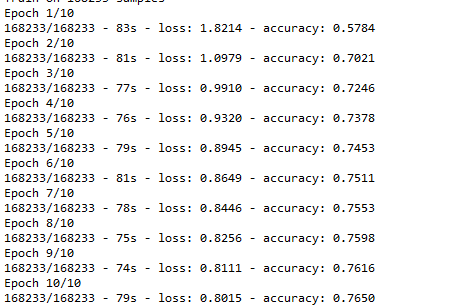
\includegraphics[width=4cm]{figures/1174003/7/praktek_15.png}
    \centering
    \caption{Illustrasi perhitungan stride 1 max pooling}
\end{figure}
\item Jelaskan kode program pada blok \# In[16]. Jelaskan arti dari setiap baris kode yang dibuat(harus beda dengan teman sekelas) dan hasil luarannya dari komputer sendiri.
\lstinputlisting[firstline=245, lastline=248]{src/1174003/7/chapter7.py}
\begin{figure}[H]
    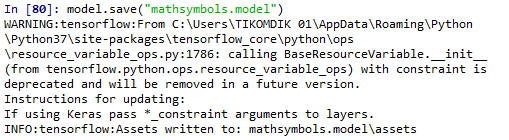
\includegraphics[width=4cm]{figures/1174003/7/praktek_16.png}
    \centering
    \caption{Illustrasi perhitungan stride 1 max pooling}
\end{figure}
\item Jelaskan kode program pada blok \# In[17]. Jelaskan arti dari setiap baris kode yang dibuat(harus beda dengan teman sekelas) dan hasil luarannya dari komputer sendiri.
\lstinputlisting[firstline=249, lastline=253]{src/1174003/7/chapter7.py}
\begin{figure}[H]
    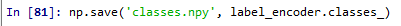
\includegraphics[width=4cm]{figures/1174003/7/praktek_17.png}
    \centering
    \caption{Illustrasi perhitungan stride 1 max pooling}
\end{figure}
\item Jelaskan kode program pada blok \# In[18]. Jelaskan arti dari setiap baris kode yang dibuat(harus beda dengan teman sekelas) dan hasil luarannya dari komputer sendiri.
\lstinputlisting[firstline=254, lastline=262]{src/1174003/7/chapter7.py}
\begin{figure}[H]
    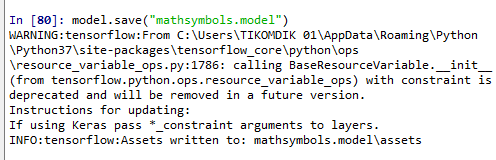
\includegraphics[width=4cm]{figures/1174003/7/praktek_18.png}
    \centering
    \caption{Illustrasi perhitungan stride 1 max pooling}
\end{figure}
\item Jelaskan kode program pada blok \# In[19]. Jelaskan arti dari setiap baris kode yang dibuat(harus beda dengan teman sekelas) dan hasil luarannya dari komputer sendiri.
\lstinputlisting[firstline=263, lastline=284]{src/1174003/7/chapter7.py}
\begin{figure}[H]
    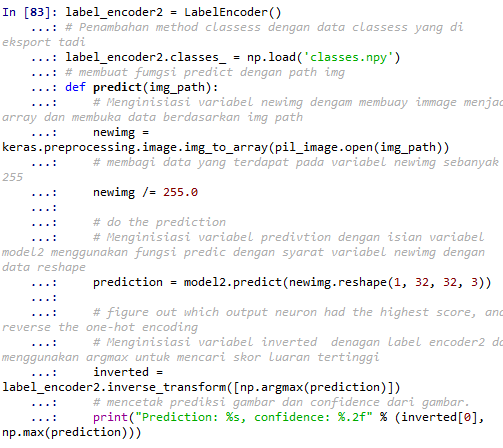
\includegraphics[width=4cm]{figures/1174003/7/praktek_19.png}
    \centering
    \caption{Illustrasi perhitungan stride 1 max pooling}
\end{figure}
\item Jelaskan kode program pada blok \# In[20]. Jelaskan arti dari setiap baris kode yang dibuat(harus beda dengan teman sekelas) dan hasil luarannya dari komputer sendiri.
\lstinputlisting[firstline=285, lastline=293]{src/1174003/7/chapter7.py}
\begin{figure}[H]
    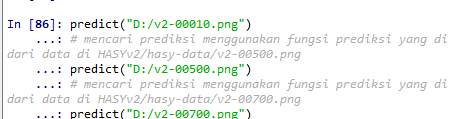
\includegraphics[width=4cm]{figures/1174003/7/praktek_20.png}
    \centering
    \caption{Illustrasi perhitungan stride 1 max pooling}
\end{figure}
\end{enumerate}
